


Ⓔ \textcolor{etc}{In this chapter we will walk through the process of downloading and running Spark in local mode on a single computer. This chapter was written for anybody who is new to Spark, including both data scientists and engineers.}

Ⓒ 本章主要介绍 Spark 的下载和本地单机模式下的运行方法。本章面向 Spark
初学者,包括数据科学家和工程师。

Ⓔ \textcolor{etc}{Spark can be used from Python, Java, or Scala. To benefit from this book, you don't need to be an expert programmer, but we do assume that you are comfortable with the basic syntax of at least one of these languages. We will include examples in all languages wherever possible.}

Ⓒ Spark 支持 Python、Java 和 Scala
语言。即便您不是专业的编程者也会从本书中受益,但我们仍然假定您已熟悉其中至少一个语言的基本语法。我们将在示例中尽量提供这三种编程语言的版本。

Ⓔ \textcolor{etc}{Spark itself is written in Scala, and runs on the Java Virtual Machine (JVM). To run Spark on either your laptop or a cluster, all you need is an installation of Java 6 or newer. If you wish to use the Python API you will also need a Python interpreter (version 2.6 or newer). Spark does not yet work with Python 3.}

Ⓒ Spark 由 Scala 语言编写而成,并需要 Java 虚拟机 (Java Virtual Machine,
JVM) 才能运行。不管是在笔记本上还是集群上运行 Spark,您都需要安装 Java 6
以上版本的编译环境。如果您想使用 Python API,还需要安装 Python
解释器(2.6 或者更高版本)。请注意 Spark 暂不支持 Python 3。


%
%%
\section{下载 Spark}\label{download-spark}

Ⓔ \textcolor{etc}{The first step to using Spark is to download and unpack it. Let's start by downloading a recent precompiled released version of Spark. Visit \emph{http://spark.apache.org/downloads.html}, select the package type of "Pre-built for Hadoop 2.4 and later", and click "Direct Download". This will download a compressed TAR file, or tarball, called spark-1.2.0-bin-hadoop2.4.tgz. }

使用Spark的第一步是下载并解压开来。我们从下载一个新近预编译版本的 Spark
开始。在浏览器中访问 \emph{http://spark.apache.org/downloads.html}
选择"Pre-built for Hadoop 2.4 and later" 安装包,点击 "Direct
Download" 下载名称为 spark-1.2.0-bin-hadoop2.4.tgz 的压缩包。

\begin{quote}
Ⓔ \textcolor{etc}{Windows users may run into issues installing Spark into a directory with a space in the name. Instead, install Spark in a directory with no space (e.g., \lstinline{C:\spark}). }
\end{quote}

\begin{quote}
Ⓒ 用户安装时可能会遇到文件夹名称中包含空格的问题,建议 Spark
的安装目录的文件夹中不包含空格,比如 \lstinline{C:\spark} 。
\end{quote}

Ⓔ \textcolor{etc}{You don't need to have Hadoop, but if you have an existing Hadoop cluster or HDFS installation, download the matching version. You can do so from \emph{http://spark.apache.org/downloads.html} by selecting a different package type, but they will have slightly different filenames. Building from source is also possible; you can find the latest source code on GitHub or select the package type of "Source Code" when downloading.}

Ⓒ 您不需要安装 Hadoop 即可运行 Spark ,但是如果您已有 Hadoop 集群或安装了 HDFS 则需要下载对应的 Spark 版本 。 您可在 \emph{http://spark.apache.org/downloads.html} 选择不同的安装包,它们的文件名会略有不同;或者在 Github 下载最新的 Spark 源代码进行编译安装。

\begin{quote}
Ⓔ \textcolor{etc}{Most Unix and Linux variants, including Mac OS X, come with a command-line tool called tar that can be used to unpack TAR files. If your operating system does not have the tar command installed, try searching the Internet for a free TAR extractor---for example, on Windows, you may wish to try 7-Zip.}
\end{quote}

\begin{quote}
Ⓒ 大多数 Unix 和 Linux 操作系统,包括 Mac OS X,都包含 tar
命令行解压工具。如果您的操作系统没有安装 tar
的命令行工具,请在互联网搜索免费的解压缩工具。比如在 Windows
系统中您可以使用 7-Zip。
\end{quote}

Ⓔ \textcolor{etc}{Now that we have downloaded Spark, let's unpack it and take a look at what comes with the default Spark distribution. To do that, open a terminal, change to the directory where you downloaded Spark, and untar the file. This will create a new directory with the same name but without the final \lstinline{.tgz} suffix. Change into that directory and see what's inside. You can use the following commands to accomplish all of that:}

Ⓔ 当Spark下载好后,解压缩可以看到Spark默认带有哪些内容。打开终端,切换至下载 Spark 的目录下将其解压。执行下面的代码将创建一个与压缩文件同名的新目录(没有\lstinline{.tgz}后缀)。使用已下语句,您可以进入该文件夹查看里面的内容:

\begin{lstlisting}
cd ~
tar -xf spark-1.2.0-bin-hadoop2.4.tgz
cd spark-1.2.0-bin-hadoop2.4
ls
\end{lstlisting}

Ⓔ \textcolor{etc}{In the line containing the \lstinline{tar} command, the \lstinline{x} flag tells \lstinline{tar} we are extracting files, and the \lstinline{f} flag specifies the name of the tarball. The \lstinline{ls} command lists the contents of the Spark directory. Let's briefly consider the names and
purposes of some of the more important files and directories you see here that come with Spark:}

Ⓒ 在 \lstinline{tar -xf spark-1.2.0-bin-hadoop2.4.tgz} 命令中,参数标签 \lstinline{x} 表示解压缩,\lstinline{f} 表示指定 \lstinline{tar} 包名称。\lstinline{ls} 命令将列出 Spark 目录下的所有文件。让我们简要介绍下 Spark 目录中的重要文件。

\textbf{\emph{README.md}}\\
Ⓔ Contains short instructions for getting started with Spark.\\
Ⓒ 包含 Spark 入门的简要说明。

\textbf{\emph{bin}}\\
Ⓔ Contains executable files that can be used to interact with Spark in
various ways (e.g., the Spark shell, which we will cover later in this
chapter).\\
Ⓒ 包含与 Spark 交互的可执行文件(如在本章后面介绍的 Spark
Shell)

\textbf{\emph{core, streaming, python, \ldots{}}}\\
Ⓔ Contains the source code of major components of the Spark project.\\
Ⓒ 包含 Spark 工程主要组件的源码

\textbf{\emph{examples}}\\
Ⓔ Contains some helpful Spark standalone jobs that you can look at and run to learn about the Spark API.\\
Ⓒ 包含可在 Spark 单机版运行的作业,您可从中了解 Spark API。

Ⓔ \textcolor{etc}{Don't worry about the large number of directories and files the Spark project comes with; we will cover most of these in the rest of this book. For now, let's dive right in and try out Spark's Python and Scala shells. We will start by running some of the examples that come with Spark. Then we will write, compile, and run a simple Spark job of our own.}

Ⓒ 读者无需对 Spark 文件夹下众多文件和目录感到困扰,本书后续章节会涵盖其中的大部分技术内容。现在,我们先深入 Spark 的 Python 和 Scala 交互式 shell。我们将从运行 Spark 官方示例开始,然后编写和运行自己的 Spark 任务。

Ⓔ \textcolor{etc} {All of the work we will do in this chapter will be with Spark running in local mode; that is, nondistributed mode, which uses only a single machine. Spark can run in a variety of different modes, or environments. Beyond local mode, Spark can also be run on Mesos, YARN, or the Standalone Scheduler included in the Spark distribution. We will cover the various deployment modes in detail in Chapter 7.}

Ⓒ 本章我们要做的是让 Spark 在本地环境下运行起来,即本地计算机非分布式的模式。 Spark 可以以不同模式在不同环境中运行。除了单机模式,Spark 还可运行于 Mesos、YARN,或在 Spark 分布式下独立调度 (Standalone Schedule) 。我们将在第七章中详细介绍各种部署模式。

\section{Introduction to Spark's Python and Scala Shells  |  Spark 的 Python 和 Scala 交互式 Shell}\label{introduction-to-sparks-python-and-scala-shells}

Ⓔ \textcolor{etc}{Spark comes with interactive shells that enable ad hoc data analysis. Spark's shells will feel familiar if you have used other shells such as those in R, Python, and Scala, or operating system shells like Bash or the Windows command prompt.}

Ⓒ Spark 的交互式 shell 支持可执行的数据分析。如果您使用其他的 shell
编程,那么您将会对 Spark shell 感觉很亲切。比如 R、Python 和 Scala
shell,以及批处理的操作系统编程或者 Windows 命令提示符。

Ⓔ \textcolor{etc}{Unlike most other shells, however, which let you manipulate data using the disk and memory on a single machine, Spark's shells allow you to interact with data that is distributed on disk or in memory across many machines, and Spark takes care of automatically distributing this processing.}

Ⓒ 与其他的 Shell只能操作单台计算机的磁盘和内存不同的是, Spark Shell支持跨多台计算机的分布式磁盘和内存计算,并且 Spark 会自动执行分布式作业处理。

Ⓔ \textcolor{etc}{Because Spark can load data into memory on the worker nodes, many distributed computations, even ones that process terabytes of data across dozens of machines, can run in a few seconds. This makes the sort of iterative, ad hoc, and exploratory analysis commonly done in shells a good fit for Spark. Spark provides both Python and Scala shells that have been augmented to support connecting to a cluster.}

Ⓒ 因为Spark将数据加载至工作节点内存中,绝大多数分布式计算甚至处理TB级的数据也仅需几秒钟。这使得Spark 适合处理迭代排序、随机和未知分析。Spark 的 Python 和 Scala 的shell 均支持集群连接。

\begin{quote}
Ⓔ \textcolor{etc}{Most of this book includes code in all of Spark's languages, but interactive shells are available only in Python and Scala. Because a shell is very useful for learning the API, we recommend using one of these languages for these examples even if you are a Java developer. The API is similar in every language.}
\end{quote}

\begin{quote}
Ⓒ 本书中大部分代码包含 Spark 支持的所有语言,但是交互式 shell 仅支持
Python 和 Scala 语言。因为 shell 是非常有效的学习 API
的方法,我们建议您使用本书中 Python 或者 Scala
语言的示例学习,即使您是一位 Java 开发者。每种语言的 API 差别都不大。
\end{quote}

Ⓔ \textcolor{etc}{The easiest way to demonstrate the power of Spark's shells is to start using one of them for some simple data analysis. Let's walk through the example from the Quick Start Guide in the official Spark documentation.}

Ⓒ 简单数据处理任务也能轻而易举的显现出Spark Shell的强大功能。让我们用
Saprk 官方文档提供的快速上手指南的案例来体验一下。

Ⓔ \textcolor{etc}{The first step is to open up one of Spark's shells. To open the Python version of the Spark shell, which we also refer to as the PySpark Shell, go into your Spark directory and type:}

Ⓒ 首先打开 Spark 交互式 shell。若要打开 Python 版本的 Spark
shell,即PySpark shell,在 Spark 目录中输入如下指令:

\begin{lstlisting}
bin/pyspark
\end{lstlisting}

Ⓔ \textcolor{etc}{(Or \lstinline{bin\pyspark} in Windows.) To open the Scala version of the shell, type:}

Ⓒ (或者在 Windows 中输入 \lstinline{bin\pyspark} ) 打开
Scala 版本的 shell,输入:

\begin{lstlisting}
bin/spark-shell
\end{lstlisting}

Ⓔ \textcolor{etc}{The shell prompt should appear within a few seconds. When the shell starts, you will notice a lot of log messages. You may need to press Enter once to clear the log output and get to a shell prompt. \emph{Figure 2-1} shows what the PySpark shell looks like when you open it.}

Ⓒ Shell 提示符会在几秒钟后出现。当 shell 启动时,您会看到很多日志消息,可以按下Enter键清除日志回到提示符。\emph{图2-1}显示了打开PySpark
shell的界面。

\begin{figure}[htbp]
\centering
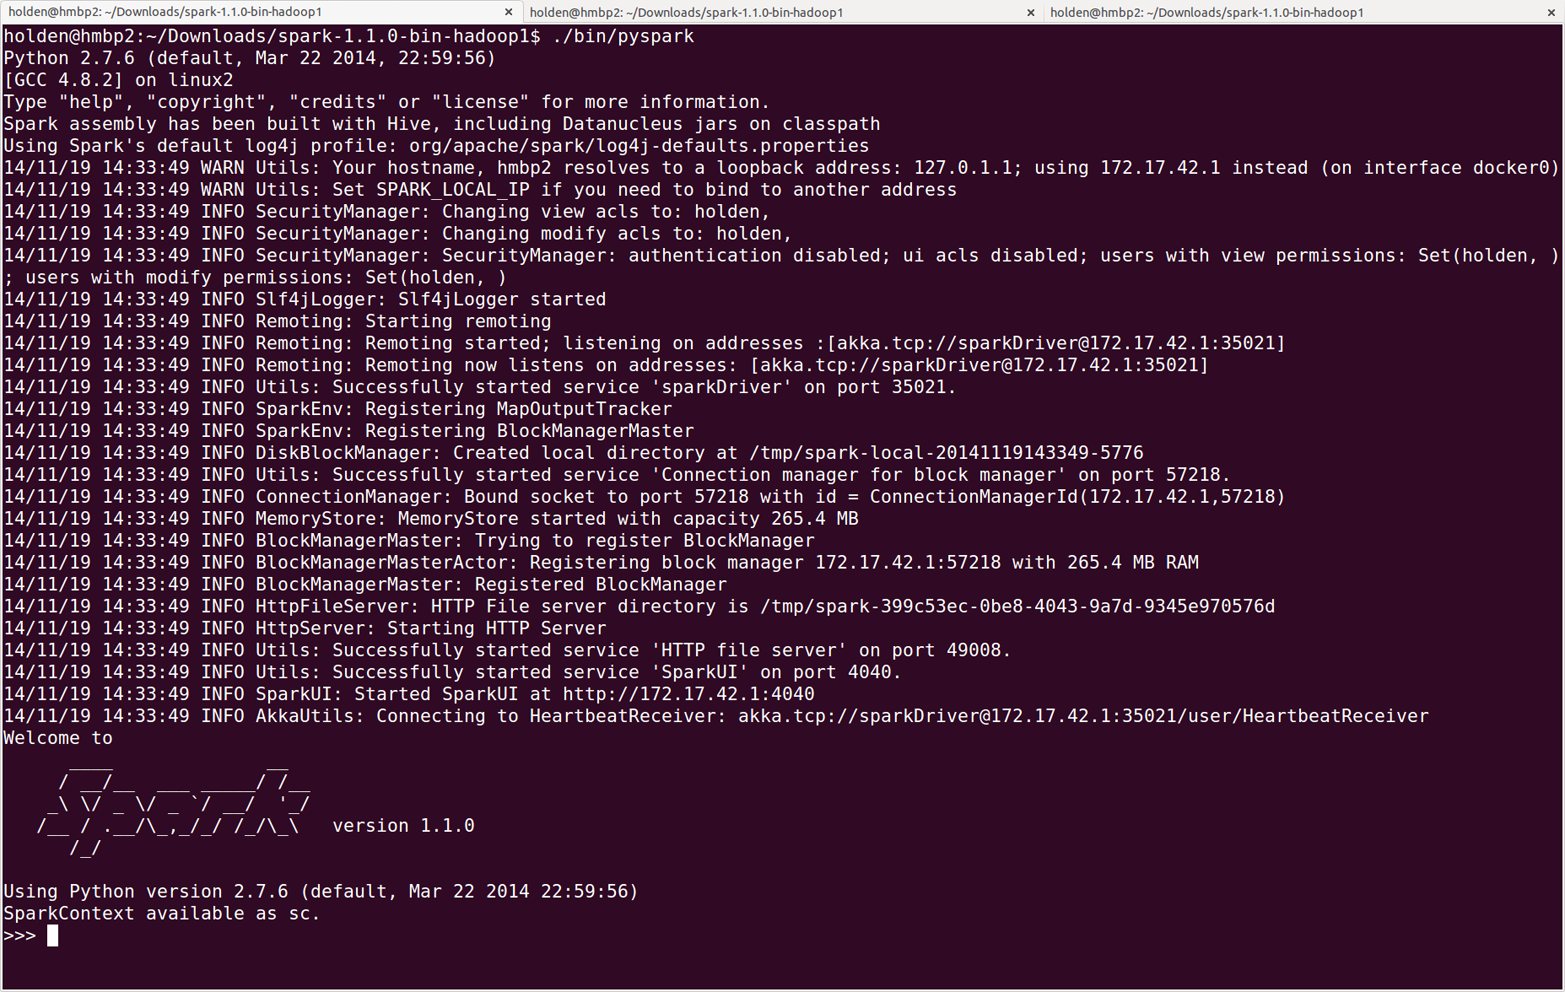
\includegraphics[width=.99\textwidth]{../images/fig_2-1.png}
\caption{The PySpark shell with default logging output  |  PySpark shell 的默认日志输出}
\end{figure}

Ⓔ \textcolor{etc}{You may find the logging statements that get printed in the shell distracting. You can control the verbosity of the logging. To do this, you can create a file in the conf directory called \lstinline{log4j.properties}. The Spark developers already include a template for this file called \lstinline{log4j.properties.template}. To make the logging less verbose, make a copy of \lstinline{conf/log4j.properties.template} called \lstinline{conf/log4j.properties} and find the following line:}

Ⓒ 在 shell 中您可以看到打印的日志信息,您也可以控制日志的详细程度。在\lstinline{conf}目录中创建名称为 \lstinline{log4j.properties} 的文件,Spark 提供了该文件的模板\lstinline{log4j.properties.template} 若不需要输出那么冗长的日志,您可以复制该模板并将其改名为 \lstinline{log4j.properties} , 在模板的复制文件中找到下面的代码:

\begin{lstlisting}
log4j.rootCategory=INFO, console
\end{lstlisting}

Ⓔ \textcolor{etc}{Then lower the log level so that we show only the WARN messages, and above by changing it to the following: }

Ⓒ 降低日志的级别只显示\textbf{警告}信息,将上面的代码修改如下:

\begin{lstlisting}
log4j.rootCategory=WARN, console
\end{lstlisting}

Ⓔ \textcolor{etc}{When you reopen the shell, you should see less output (Figure 2-2). }

Ⓒ 重新打开 shell,您可以看见输出信息减少了。

\begin{figure}[htbp]
\centering
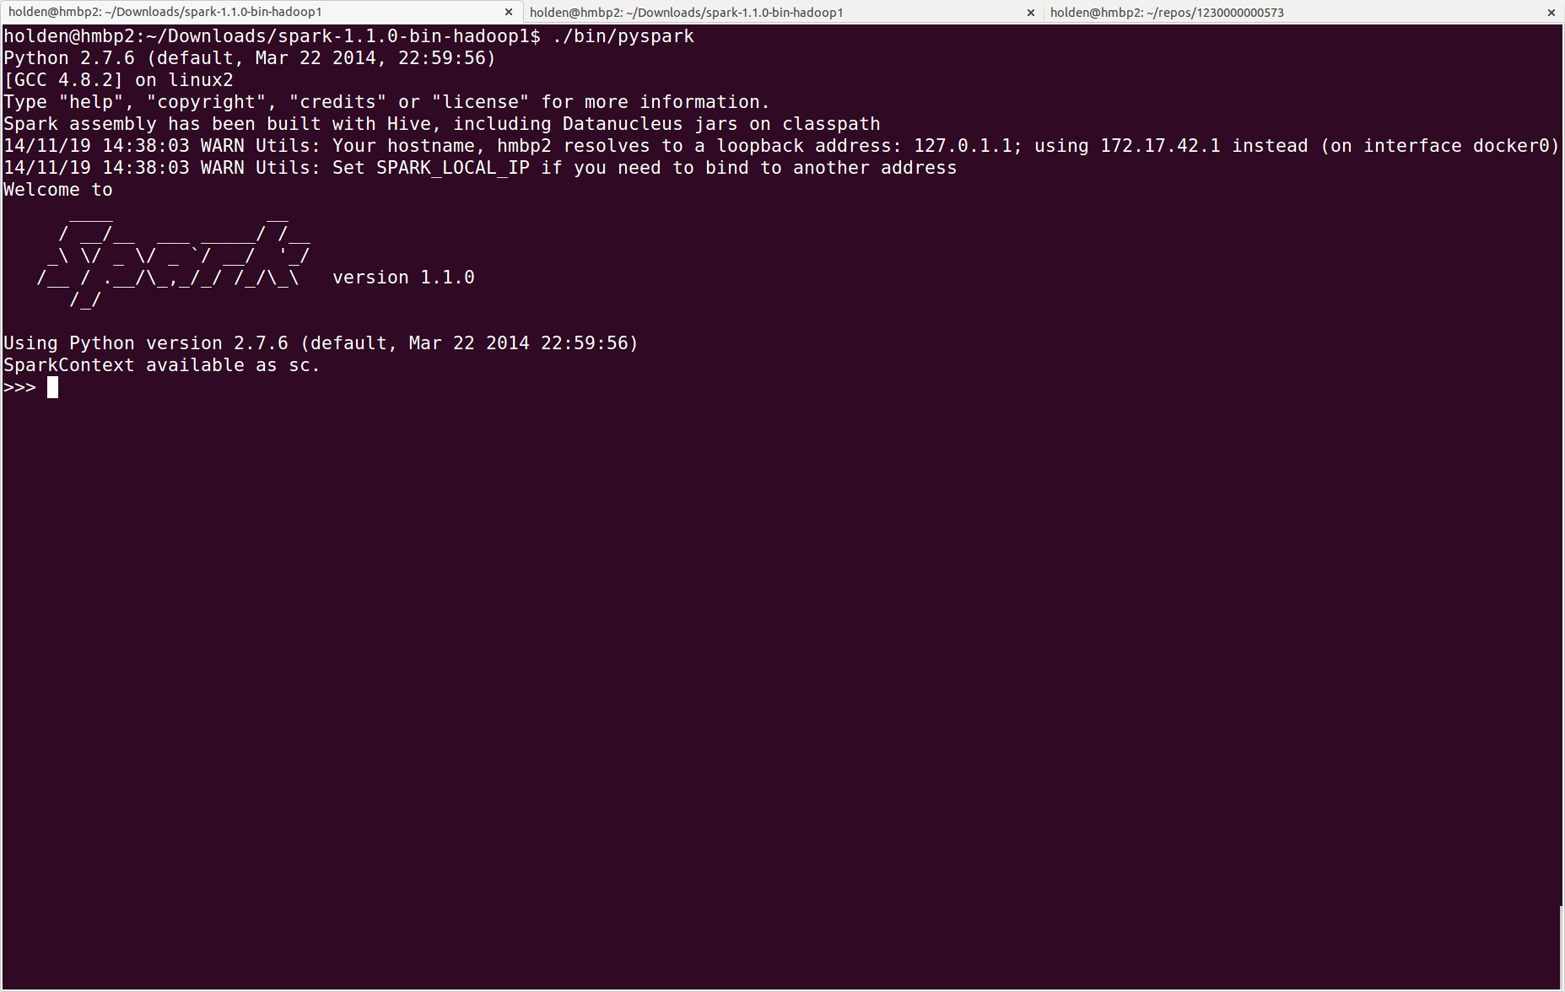
\includegraphics[width=.99\textwidth]{../images/fig_2-2.png}
\caption{The PySpark shell with less logging output  |  PySpark shell输出信息减少}
\end{figure}


\begin{center}\rule{0.5\linewidth}{\linethickness}\end{center}

\begin{quote}
Ⓔ \textcolor{etc}{\textbf{Using IPython} IPython is an enhanced Python shell that many Python users prefer, offering features such as tab completion. You can
find instructions for installing it at http://ipython.org. You can use IPython with Spark by setting the IPYTHON environment variable to 1:}
\end{quote}

\begin{lstlisting}
IPYTHON=1 ./bin/pyspark
\end{lstlisting}

Ⓔ \textcolor{etc}{To use the IPython Notebook, which is a web-browser-based version of IPython, use:}

\begin{lstlisting}
IPYTHON_OPTS="notebook" ./bin/pyspark
\end{lstlisting}

Ⓔ \textcolor{etc}{On Windows, set the variable and run the shell as follows:}
\lstinline{set IPYTHON=1 bin\pyspark}

\begin{center}\rule{0.5\linewidth}{\linethickness}\end{center}

\begin{quote}
Ⓒ \textbf{使用 IPython} IPython 是颇受 python 使用者喜爱的增强版 Python
shell,提供诸如 tab 键自动补全功能。更多信息请查看http://ipython.org
。将 IPYTHON 的环境变量设置为 1 即可在 Spark 中使用 \lstinline{IPython}。
\end{quote}

\begin{lstlisting}
IPYTHON=1 ./bin/pyspark
\end{lstlisting}

若要使用基于浏览器的 IPython Notebook,请使用如下命令:

\begin{lstlisting}
IPYTHON_OPTS="notebook" ./bin/pyspark
\end{lstlisting}

在 Windows 中设置变量的方法如下:
\lstinline{set IPYTHON=1 bin\pyspark}

\begin{center}\rule{0.5\linewidth}{\linethickness}\end{center}

Ⓔ \textcolor{etc}{In Spark, we express our computation through operations on distributed collections that are automatically parallelized across the cluster. These collections are called resilient distributed datasets, or RDDs. RDDs are Spark's fundamental abstraction for distributed data and computation.}

Ⓒ 在 Spark 中我们的计算时通过对集群间自动并行的分布式集合上进行操作的,这些集合被称为弹性分布数据集(resilient distributed datasets, RDDs)。RDD 是 Spark 做分布式数据和计算的基本抽象概念。

Ⓔ \textcolor{etc}{Before we say more about RDDs, let's create one in the shell from a local text file and do some very simple ad hoc analysis by following \emph{Example 2-1} for Python or \emph{Example 2-2} for Scala.}

Ⓒ 在详细探讨 RDD 之前,我们先创建一个 shell
程序读取本地文本文件并计算简单的特定分析。下面的\emph{示例 2-1}
用于Python语音,\emph{示例 2-2}用于Scala语言。

\emph{Example 2-1. Python line count \textbar{} 示例 2-1. Python line
count} \label{exmp2-1}

\begin{lstlisting}
>>> lines = sc.textFile("README.md") # Create an RDD called lines
>>> lines.count() # Count the number of items in this RDD
>>> lines.first() # First item in this RDD, i.e. first line of
README.md u'# Apache Spark'
\end{lstlisting}

\emph{Example 2-2. Scala line count \textbar{} 示例 2-2. Scala line
count} \label{exmp2-2}

\begin{lstlisting}
scala> val lines = sc.textFile("README.md") // Create an RDD
called lines lines: spark.RDD[String] = MappedRDD[...]
scala> lines.count() // Count the number of items in
this RDD res0: Long = 127
scala> lines.first() // First item in this RDD, i.e. first line of
README.md res1: String = # Apache Spark
\end{lstlisting}

Ⓔ To exit either shell, press \lstinline{Ctrl-D}. Ⓒ 若要退出 shell,按下
\lstinline{Ctrl-D}。

\begin{quote}
\textcolor{etc}{ We will discuss it more in Chapter 7, but one of the messages you may have noticed is \lstinline{INFO SparkUI: Started SparkUI at http://{[}ipaddress{]}:4040}. You can access the Spark UI there and see all sorts of information about your tasks and cluster.}
\end{quote}

\begin{quote}
我们会在第七章中详细讨论。但是您可能已经注意到一条消息:\lstinline{INFO SparkUI:  Started  SparkUI at http://{[}ipaddress{]}:4040}
。您可以通过此 Spark UI 看见 更多任务和集群的信息。
\end{quote}

Ⓔ \textcolor{etc}{In \hyperref[exmp2-1]{Examples 2-1} and \hyperref[exmp2-2]{2-2}, the variable called lines is an RDD, created here from a text file on our local machine. We can run various parallel operations on the RDD, such as counting the number of elements in the dataset (here, lines of text in the file) or printing the first one. We will discuss RDDs in great depth in later chapters, but before we go any further, let's take a moment now to introduce basic Spark concepts.}

Ⓒ 在\hyperref[exmp2-1]{示例 2-1} 和\hyperref[exmp2-2]{2-2} 中,变量 lines 为
RDD,它是在本地机器中读取文本文件后被创建的。我们可以对此 RDD
运行各种并行操作,比如在数据集(这里指文件中文本的行数)中统计元素的数量,或者打印元素。在后面的章节中我们将深入讨论
RDD,在这个之前我们花点时间介绍 Spark 的基本概念。

\section{Introduction to Core Spark Concepts  |  Spark 核心概念综述}\label{introduction-to-core-spark-concepts-}

Ⓔ \textcolor{etc}{Now that you have run your first Spark code using the shell, it's time to learn about programming in it in more detail.}

Ⓒ 现在您已经在 shell 中运行了第一个 Spark 代码,是时候更深入学习编程了。

Ⓔ \textcolor{etc}{At a high level, every Spark application consists of a driver program that launches various parallel operations on a cluster. The driver program contains your application's main function and defines distributed datasets on the cluster, then applies operations to them. In the preceding examples, the driver program was the Spark shell itself, and you could just type in the operations you wanted to run.}

Ⓒ 每一个 Spark 应用程序都包含一个在集群上运行各种并行操作的驱动程序,驱动程序包含应用程序的主函数和定义在集群上的分布式数据集。在前面的示例中,驱动程序就是 Spark shell 本身,您只需输入您想要执行的操作即可。

Ⓔ \textcolor{etc}{ Driver programs access Spark through a \lstinline{SparkContext} object, which represents a connection to a computing cluster. In the shell, a SparkContext is automatically created for you as the variable called \lstinline{sc}. Try printing out \lstinline{sc} to see its type, as shown in \hyperref[exmp2-3]{\emph{Example 2-3}}.}

Ⓒ 驱动程序通过一个链接到计算集群上的 \lstinline{SparkContext} 对象访问
Spark 计算集群,在 shell 中,SparkContext 被自动创建为名称是 \lstinline{sc}
的变量,在\hyperref[exmp2-3]{\emph{示例 2-3}}中我们输入 \lstinline{sc},则 shell 显示其类型。

\emph{Example 2-3. Examining the sc variable  |  示例 2-3. 检视sc变量} \label{exmp2-3}

\begin{lstlisting}
>>> sc
<pyspark.context.SparkContext object at 0x1025b8f90>
\end{lstlisting}

Ⓔ \textcolor{etc}{Once you have a \lstinline{SparkContext}, you can use it to build RDDs. In \hyperref[exmp2-1]{\emph{Examples 2-1}} and \hyperref[exmp2-1]{\emph{2-2}}, we called \lstinline{sc.textFile()} to create an RDD representing the lines of text in a file. We can then run various operations on these lines, such as \lstinline{count()}.}

Ⓒ 在创建了 \lstinline{SparkContext} 对象之后,您就可创建 RDD 了。在 \hyperref[exmp2-1]{\emph{示例 2-1}} 和 \hyperref[exmp2-2]{\emph{2-2}} 中,我们调用 \lstinline{sc.textFile()} 创建一个代表文件中文本行数的 RDD。然后,我们就可以在这些行上进行各种操作,例如 \lstinline{count()}。

Ⓔ \textcolor{etc}{To run these operations, driver programs typically manage a number of nodes called executors. For example, if we were running the count() operation on a cluster, different machines might count lines in different ranges of the file. Because we just ran the Spark shell locally, it executed all its work on a single machine---but you can connect the same shell to a cluster to analyze data in parallel. Figure 2-3 shows how Spark executes on a cluster.}

Ⓒ 若要运行这些操作,驱动程序通常管理者多个拥有 \lstinline{executor} 的工作节点。比如,我们在集群中执行 \lstinline{count()} 操作,不同的机器可能计算 lines 变量不同的部分。我们只在本地运行 Spark shell,则它被执行在单机中,如果我们将 shell 连接至集群它也可并行的分析数据。\emph{图 2-3} 展示了 Spark 如何在集群上执行。


% FIGURE 2-3
\begin{figure}[htbp]
\centering
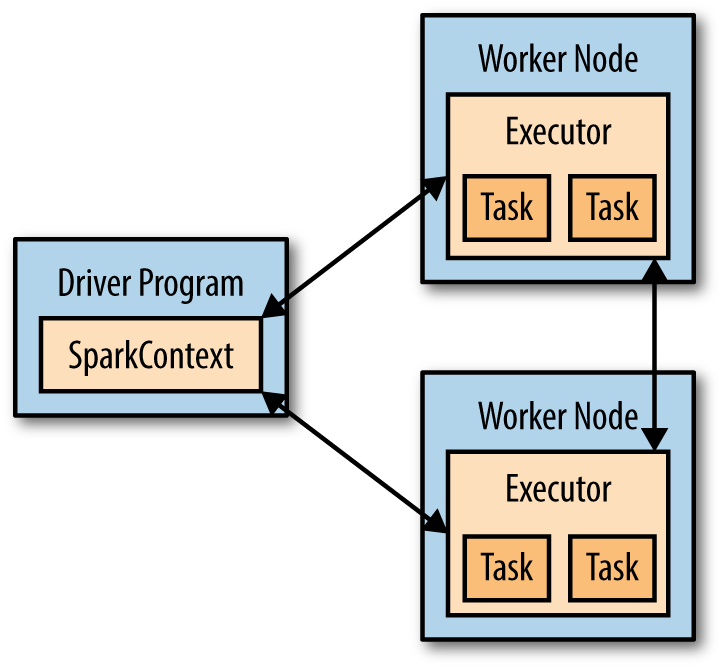
\includegraphics[width=.6\textwidth]{../images/fig_2-3.png}
\caption{Components for distributed execution in Spark  |  }
\end{figure} \label{fig2-3}

Ⓔ \textcolor{etc}{Finally, a lot of Spark's API revolves around passing functions to its operators to run them on the cluster. For example, we could extend our README example by filtering the lines in the file that contain a word, such as Python, as shown in Example 2-4 (for Python) and Example 2-5 (for Scala).}

Ⓒ Spark 的 API 很大程度上依靠在驱动程序里传递函数到集群上运行。比如,我们扩展上面的 README 示例,筛选文本中包含的特定关键词``Python''的行,代码如\emph{示例2-4}(Python),\emph{示例 2-5}(Scala)。

\emph{Example 2-4. Python filtering example \textbar{}\textbar{} 示例
2-4 Python filtering example}

\begin{lstlisting}
>>> lines = sc.textFile("README.md")
>>> pythonLines = lines.filter(lambda line: "Python" in line)
>>> pythonLines.first() u'## Interactive Python Shell'
\end{lstlisting}

\emph{Example 2-5. Scala filtering example} \emph{示例 2-5. Scala
filtering example}

\begin{lstlisting}
scala> val lines = sc.textFile("README.md") // Create an RDD
called lines lines: spark.RDD[String] = MappedRDD[...]
\end{lstlisting}

\begin{lstlisting}
scala> val pythonLines = lines.filter(line =>
line.contains("Python")) pythonLines: spark.RDD[String] = FilteredRDD[...]
\end{lstlisting}

\begin{lstlisting}
scala> pythonLines.first() res0:
String = ## Interactive Python Shell
\end{lstlisting}

\begin{center}\rule{0.5\linewidth}{\linethickness}\end{center}

\begin{quote}
Ⓔ \textcolor{etc}{\textbf{Passing Functions to Spark} \\
If you are unfamiliar with the lambda or =\textgreater{} syntax in Examples 2-4 and 2-5, it is a shorthand way to define functions inline in Python and Scala. When using Spark in these languages, you can also define a function separately and then pass its name to Spark. For example, in Python:}

\begin{lstlisting}
def hasPython(line):
  return "Python" in line
pythonLines = lines.filter(hasPython)
\end{lstlisting}

Ⓔ \textcolor{etc}{Passing functions to Spark is also possible in Java, but in this case they are defined as classes, implementing an interface called Function . For example:}

\begin{lstlisting}
JavaRDD<String> pythonLines = lines.filter(
  new Function<String, Boolean>() {
    Boolean call(String line) { return line.contains("Python"); }
    }
  );
\end{lstlisting}

Ⓔ \textcolor{etc}{Java 8 introduces shorthand syntax called lambdas that looks similar to Python and Scala. Here is how the code would look with this syntax:}

\begin{lstlisting}
JavaRDD<String> pythonLines = lines.filter(line -> line.contains("Python"));
\end{lstlisting}

Ⓔ \textcolor{etc}{We discuss passing functions further in "Passing Functions to Spark" on page 30.}
\end{quote}

\begin{quote}

Ⓒ \textbf{Spark 传递函数}\\
如果您不熟悉示例 2-4 和 2-5 中的 lambda 表达式 或者 =\textgreater{}
语法,那么在 此说明其实它是在 Python 和 Scala
中的定义内联函数的简短写法。如果您 在 Spark
中使用这些语言,您可定义函数然后将其名称传递给 Spark。比 如,在 Python
语言中:

\begin{lstlisting}
def hasPython(line):
return "Python" in line
pythonLines = lines.filter(hasPython)
\end{lstlisting}

Spark 传递函数也支持 Java 语言,但在此情况下传递函数被定义为类,实
现调用函数的接口。比如:

\begin{lstlisting}
JavaRDD<String> pythonLines = lines.filter(
  new Function<String, Boolean>() {
    Boolean call(String line) { return
    line.contains("Python"); }
    }
  );
\end{lstlisting}

Java 8 引入了调用了 lambda 的的简短写法,与 Python 和 Scala 很类
似。这种写法的句式会像这样:

\begin{lstlisting}
JavaRDD<String> pythonLines = lines.filter(line ->
line.contains("Python"));
\end{lstlisting}

我们将在 30 页的 "Spark 传递函数"中深入讨论传递函数。

\end{quote}


Ⓔ \textcolor{etc}{While we will cover the Spark API in more detail later, a lot of its magic is that function-based operations like filter also parallelize
across the cluster. That is, Spark automatically takes your function
(e.g., \lstinline{line.contains("Python")}) and ships it to executor nodes. Thus, you can write code in a single driver program and automatically have
parts of it run on multiple nodes. Chapter 3 covers the RDD API in
detail.}

Ⓒ Spark API
包含许多魅力无穷的基于函数的操作可基于集群并行计算,比如筛选(filter)操作,我们在后面的章节详细介绍。Spark
自动将您的函数传递给执行(executor)节点。因此,您可在单独的驱动程序中编写代码,它会自动的在多个节点中运行。本书第三章涵盖了
RDD API 的详细介绍。

\subsection{Standalone Applications  |  独立应用程序} \label{standalone-applications}

Ⓔ \textcolor{etc}{The final piece missing in this quick tour of Spark is how to use it in standalone programs. Apart from running interactively, Spark can be linked into standalone applications in either Java, Scala, or Python. The main difference from using it in the shell is that you need to initialize your own SparkContext. After that, the API is the same.}

Ⓒ Spark 快速入门教程中缺少如何在独立(Standalone)应用程序中使用
Spark,其实 Spark 除了可以交互式 shell 运行,还可以在 Java、Scala 和
Python 的独立应用程序中依赖 Spark 运行。唯一与 shell
不同的是,独立应用程序中需要初始化 SparkContext,除此之外所有的 API
都是相同的。

Ⓔ \textcolor{etc}{The process of linking to Spark varies by language. In Java and Scala, you give your application a Maven dependency on the \lstinline{spark-core} artifact. As of the time of writing, the latest Spark version is 1.2.0, and the Maven coordinates for that are:

Ⓒ 在独立应用程序中依赖 Spark 的方法因语言而异。在 Java 和 Scala
中,您可在设置 Spark 核心的 Maven 依赖。随着本书版本的书写,最新的 spark
版本为 1.2.0,相应的 Maven 依赖设置为:

\begin{lstlisting}
groupId = org.apache.spark
artifactId = spark-core_2.10
version = 1.2.0
\end{lstlisting}

Ⓔ \textcolor{etc}{Maven is a popular package management tool for Java-based languages that lets you link to libraries in public repositories. You can use Maven itself to build your project, or use other tools that can talk to the Maven repositories, including Scala's sbt tool or Gradle. Popular integrated development environments like Eclipse also allow you to directly add a Maven dependency to a project.}

Ⓒ Maven 是受欢迎的基于 Java 语言的包管理工具,可以链接至公共的资源库。您可以使用 Maven
创建自己的应用程序,也可以其他的工具比如 Scala 的 sbt 或者 Gradle
创建。流行的集成开发环境如 Eclipse 允许直接添加 Maven 依赖至 工程中。

Ⓔ \textcolor{etc}{In Python, you simply write applications as Python scripts, but you must run them using the bin/spark-submit script included in Spark. The spark-submit script includes the Spark dependencies for us in Python. This script sets up the environment for Spark's Python API to function. Simply run your script with the line given in Example 2-6.}

Ⓒ 在 Python 中,您可编写 Python 脚本的应用程序,然后使用
\lstinline{bin/sparksubmit} 提交 脚本至 Spark 运行。在 spark-submit
脚本中包含供 Python 使用的 Spark 依赖,在此脚本中设置 Spark 的 Python
API 的运行环境。

\emph{Example 2-6. Running a Python script  | 示例 2-6 运行 Python 脚本}

\begin{lstlisting}
bin/spark-submit my_script.py
# (请注意在 Windows 中使用反斜杠\替代正斜杠/。)
\end{lstlisting}

\subsection{Initializing a SparkContext  |  初始化 SparkContext}\label{initializing-a-sparkcontext}

Ⓔ \textcolor{etc}{Once you have linked an application to Spark, you need to import the Spark packages in your program and create a \lstinline{SparkContext}. You do so by first creating a \lstinline{SparkConf} object to configure your application, and then building a \lstinline{SparkContext} for it. \emph{Examples 2-7} through \emph{2-9} demonstrate this in each supported language.}

Ⓒ 如果您将应用程序链接至 Spark,则需在应用程序中引入 Spark
包并创建\lstinline{SparkContext}。首先创建 \lstinline{SparkConf}
对象配置应用程序,然后实例化\lstinline{SparkContext}。\emph{示例 2-7} 到
\emph{2-9} 以三种语言展示初始化 \lstinline{SparkContext} 的方法。

\emph{Example 2-7. Initializing Spark in Python}

\begin{lstlisting}
from pyspark import SparkConf, SparkContext
conf = SparkConf().setMaster("local").setAppName("My App")
sc = SparkContext(conf = conf)
\end{lstlisting}

\emph{Example 2-8. Initializing Spark in Scala}

\begin{lstlisting}
import org.apache.spark.SparkConf
import org.apache.spark.SparkContext
import org.apache.spark.SparkContext._
val conf = new SparkConf().setMaster("local").setAppName("My App")
val sc = new SparkContext(conf)
\end{lstlisting}

\emph{Example 2-9. Initializing Spark in Java}

\begin{lstlisting}
import org.apache.spark.SparkConf;
import org.apache.spark.api.java.JavaSparkContext;
SparkConf conf = new SparkConf().setMaster("local").setAppName("My App");
JavaSparkContext sc = new JavaSparkContext(conf);
\end{lstlisting}

Ⓔ \textcolor{etc}{These examples show the minimal way to initialize a SparkContext, where you passtwo parameters: • A cluster URL, namely local in these examples, which tells Spark how to connectto a cluster. local is a special value that runs Spark on one thread on the local machine, without connecting to a cluster. • An application name, namely My App in these examples. This will identify your application on the cluster manager's UI if you connect to a cluster.}

Ⓒ 这些示例展示最简单的初始化 SparkContext 的方法,其中传递了两个参数: •
集群URL参数,代表Spark连接到集群的方式,本例中设定为local,表示 Spark
线程仅运行于本地机器而非连接至集群。 • 应用程序名称参数,本例中被定义为
My App,如果您连接至集群,可在集群管理的 UI
界面中通过应用的名称找到您自己的应用程序。

Ⓔ \textcolor{etc}{Additional parameters exist for configuring how your application executes or adding code to be shipped to the cluster, but we will cover these in later chapters of the book.}

Ⓒ
关于应用程序执行或者提交至集群的附加参数配置,将在本书后面的章节中介绍。

Ⓔ \textcolor{etc}{After you have initialized a SparkContext, you can use all the methods we showed before to create RDDs (e.g., from a text file) and manipulate them.}

Ⓒ 在您初始化 SparkContext 之后,即可调用我们之前展示给您的所有方法来创建
RDD(比如从文本文件读取)并操纵他们。

Ⓔ \textcolor{etc}{Finally, to shut down Spark, you can either call the \lstinline{stop()} method on your Spark-Context, or simply exit the application (e.g., with \lstinline{system.exit(0)} or \lstinline{sys.exit()}).}

Ⓒ 最后,您可调用 \lstinline{stop()} 方法关闭 Spark,或者简单的退出该应用程序(比如\lstinline{System.exit(0)} 或者 \lstinline{sys.exit()} )。

Ⓔ \textcolor{etc}{This quick overview should be enough to let you run a standalone Spark application on your laptop. For more advanced configuration, Chapter 7 will cover how to connect your application to a cluster, including packaging your application so that its code is automatically shipped to worker nodes. For now, please refer to the Quick Start Guide in the official Spark documentation.}

Ⓒ 以上足以让您在笔记本电脑上运行一个单机(Standalone)的 Spark
应用程序。对于更高级的配置,第七章中将介绍如何将应用程序连接至集群,以及如何将应用程序打包以便代码自动提交至工作节点。目前,我们还是参照
Spark 官方文档的快速入门。

\subsection{创建独立(Standalone)应用程序}\label{ux521bux5efaux72ecux7acbstandaloneux5e94ux7528ux7a0bux5e8f}

Ⓔ \textcolor{etc}{This wouldn't be a complete introductory chapter of a Big Data book if we didn't have a word count example. On a single machine, implementing word count is simple, but in distributed frameworks it is a common example because it involves reading and combining data from many worker nodes. We will look at building and packaging a simple word count example with both sbt and Maven. All of our examples can be built together, but to illustrate a stripped-down build with minimal dependencies we have a separate smaller project underneath the \lstinline{learning-spark-examples/mini-complete-example} directory, as you can see in \emph{Examples 2-10} (Java) and \emph{2-11} (Scala).

Ⓒ
如果本章没有字数统计的示例,那么就不是完整大数据图书的导论章节。在单机中运行字数统计的程序很简单,但是在分布式框架中它却是一个常见的示例,因为他需要在众多的工作节点中读取和合并数据。接下来我们分别以 sbt 和 Maven
的方式创建和打包简单的字数统计的示例。我们所有的示例本都可以一起编译,但是为了说明这种最小依赖的精简编译方式,我们将其分解为多个小的程序,代码示例在目录
\lstinline{learning-sparkexamples/mini-complete-example}下,您可参阅示例
\emph{2-10}(Java)和 \emph{2-11}(Scala)。

Ⓔ Example 2-10. Word count Java application---don't worry about the
details yet

\begin{lstlisting}
// Create a Java Spark Context
SparkConf conf = new SparkConf().setAppName("wordCount");
JavaSparkContext sc = new JavaSparkContext(conf);
// Load our input data.
JavaRDD<String> input = sc.textFile(inputFile);
// Split up into words.
JavaRDD<String> words = input.flatMap(
  new FlatMapFunction<String, String>() {
    public Iterable<String> call(String x) {
      return Arrays.asList(x.split(" "));
}});
// Transform into pairs and count.
JavaPairRDD<String, Integer> counts = words.mapToPair(
  new PairFunction<String, String, Integer>(){
    public Tuple2<String, Integer> call(String x){
      return new Tuple2(x, 1);
    }}).reduceByKey(new Function2<Integer, Integer, Integer>(){
        public Integer call(Integer x, Integer y){ return x + y;}});
// Save the word count back out to a text file, causing evaluation.
counts.saveAsTextFile(outputFile);
\end{lstlisting}

Ⓔ Example 2-11. Word count Scala application---don't worry about the
details yet

\begin{lstlisting}
// Create a Scala Spark Context. val conf = new
SparkConf().setAppName("wordCount")
val sc = new SparkContext(conf)
// Load our input data.
val input = sc.textFile(inputFile)
// Split it up into words.
val words = input.flatMap(line => line.split(" "))
// Transform into pairs and count.
val counts = words.map(word => (word, 1)).reduceByKey{case (x, y) => x + y}
// Save the word count back out to a text file, causing evaluation.
counts.saveAsTextFile(outputFile)
\end{lstlisting}

Ⓔ \textcolor{etc}{We can build these applications using very simple build files with both sbt (\emph{Example 2-12}) and Maven (\emph{Example 2-13}). We've marked the Spark Core dependency as provided so that, later on, when we use an assembly JAR we don't include the spark-core JAR, which is already on the classpath of the workers.}

Ⓒ 我们可以使用非常简单的编译文件比如 sbt(\emph{示例 2-12})和 Maven
(\emph{示例 2-13})创建应用程序。我们以 provided 标签标记了 Spark
的核心依赖,以便在稍后的编程中我们可以使用该程序集,而不必导入
spark-coreJAR包。

\begin{itemize}
\item
  Example 2-12. sbt build file *

\begin{lstlisting}
name := "learning-spark-mini-example"
version := "0.0.1"
scalaVersion := "2.10.4"
// additional libraries
libraryDependencies ++= Seq(
"org.apache.spark" %% "spark-core" % "1.2.0" % "provided"
)
\end{lstlisting}
\item
  Example 2-13. Maven build file *

\begin{lstlisting}
<project>
<groupId>com.oreilly.learningsparkexamples.mini</groupId> <artifactId>learning-spark-mini-example</artifactId>
<modelVersion>4.0.0</modelVersion>
<name>example</name>
<packaging>jar</packaging>
<version>0.0.1</version>
<dependencies>
<dependency> <!-- Spark dependency -->
<groupId>org.apache.spark</groupId>
<artifactId>spark-core_2.10</artifactId>
<version>1.2.0</version>
<scope>provided</scope>
</dependency>
</dependencies>
<properties>
<java.version>1.6</java.version>
</properties>
<build>
<pluginManagement>
<plugins>
<plugin>
<groupId>org.apache.maven.plugins</groupId>
<artifactId>maven-compiler-plugin</artifactId>
<version>3.1</version>
<configuration>
<source>${java.version}</source>
<target>${java.version}</target>
</configuration>
</plugin>
</plugins>
</pluginManagement>
</build>
</project>
\end{lstlisting}
\end{itemize}

\begin{quote}
Ⓔ \textcolor{etc}{ The spark-core package is marked as provided in case we package our application into an assembly JAR. This is covered in more detail in
Chapter 7. }
\end{quote}

\begin{quote}
Ⓒ spark-core 包已经被标记为 provided,在应用程序打包时将自动引入该 JAR
包。更详细的内容在第七章中介绍。
\end{quote}

Ⓔ \textcolor{etc}{Once we have our build defined, we can easily package and run our application using the bin/spark-submit script. The spark-submit script sets up a number of environment variables used by Spark. From the mini-complete-example directory we can build in both Scala (Example 2-14) and Java (Example 2-15).}

Ⓒ
一旦有了自己的编译定义文件,我们可以轻松的将应用程序打包并使用bin/spark-submit
脚本运行。 bin/spark-submit 脚本包含设置 Spark
运行的环境变量参数。在目录中我们可以编译
Scala(示例2-14)和Java(示例2-15)应用。

Example 2-14. Scala build and run

\begin{lstlisting}
sbt clean package
$SPARK_HOME/bin/spark-submit \
--class com.oreilly.learningsparkexamples.mini.scala.WordCount \
./target/...(as above) \
./README.md  ./wordcounts
\end{lstlisting}

Example 2-15. Maven build and run

\begin{lstlisting}
mvn clean && mvn compile && mvn package
$SPARK_HOME/bin/spark-submit \ --class
com.oreilly.learningsparkexamples.mini.java.WordCount
\ ./target/learning-spark-mini-example-0.0.1.jar \
./README.md ./wordcounts
\end{lstlisting}

Ⓔ \textcolor{etc}{For even more detailed examples of linking applications to Spark, refer to the Quick Start Guide in the official Spark documentation. Chapter 7 covers packaging Spark applications in more detail.}

Ⓒ 更详细的 Spark 应用程序的示例请参阅 Spark
官方文档的快速入门。第七章也将详细介绍 Spark 应用程序的打包方法。

\section{结论}\label{ux7ed3ux8bba}

Ⓔ \textcolor{etc}{In this chapter, we have covered downloading Spark, running it locally on your laptop, and using it either interactively or from a standalone application. We gave a quick overview of the core concepts involved in programming with Spark: a driver program creates a SparkContext and RDDs, and then runs parallel operations on them. In the next chapter, we will dive more deeply into how RDDs operate.}

Ⓒ 本章我们介绍了下载
Spark,在笔记本电脑中本地运行,使用交互式方法和以独立应用程序的方式运行
Spark。并简要展示了涉及 Spark
编程的核心概念:在驱动程序中创建SparkContext 和
RDD,然后执行并行计算的操作。在下一章节中我们将深入介绍 RDD 的操作。

